\documentclass[a4paper,addpoints]{exam}

\usepackage{commath}
\usepackage{siunitx}

% russian integral
\usepackage{scalerel}
\DeclareMathOperator*{\rint}{\scalerel*{\rotatebox{17}{$\!\int\!$}}{\int}}

\qformat{\textbf{\large{Question \thequestion}}\hfill}
\pointsinrightmargin

\begin{document}

\begin{coverpages}

\begin{center}
  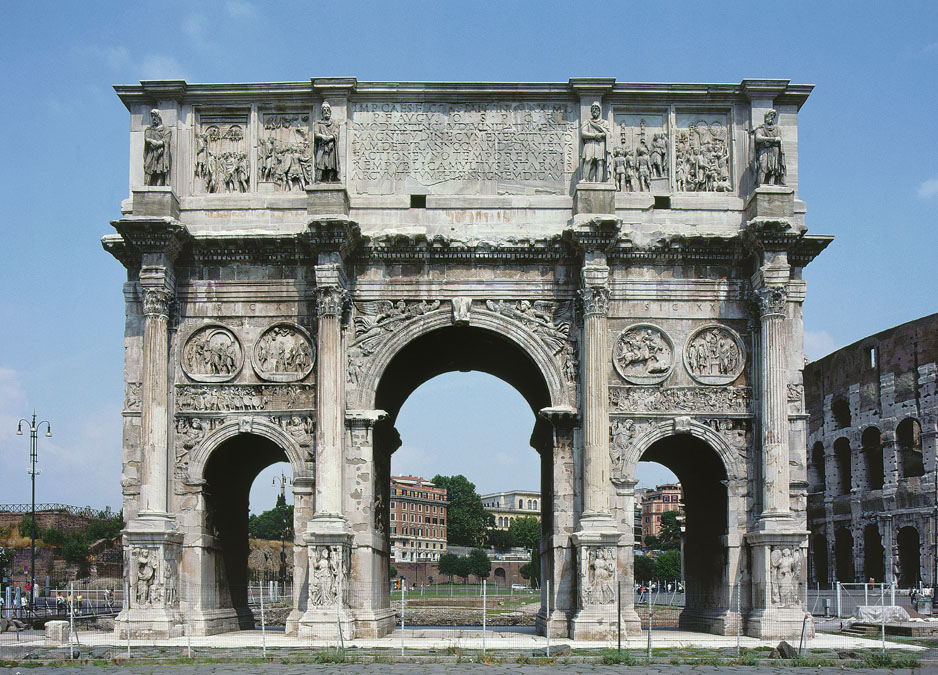
\includegraphics[width=0.6\textwidth]{exam-cover-03}

  \vspace{5mm}

  \textbf{\Huge{Level Three Calculus}}

  \vspace{2mm}

  \textbf{\Huge{Differentiation}}
\end{center}

\vspace{5mm}

\noindent
\large{There are three questions, worth a total of \numpoints\ marks.\\
       Attempt ALL questions, showing all working.\\
       Read questions carefully before attempting them.\\
       Marks are available for partial answers.\\
       The amount of time expected to be spent per question may not necessarily correlate ``nicely'' to the number of marks.\\
       Diagrams may be used to support answers.\\
       Candidates who do not provide diagrams for some questions may be disadvantaged.\\
       Some marks are given for clarity and neatness of solutions or proofs.}
\vspace{2mm}

\begin{tabular}{ll}
  \textbf{Time Allowed:}& One Hour\\
  \textbf{Achieved:}& 11 marks\\
  \textbf{Merit:}& 19 marks\\
  \textbf{Excellence:}& 27 marks
\end{tabular}

\vfill

\begin{center}
  \gradetable[h][questions]
  \vspace{2mm}

  \textbf{Available Grades:} \textit{Not Achieved}\quad\textit{Achieved}\quad\textit{Merit}\quad\textit{Excellence}
\end{center}

\end{coverpages}

\begin{questions}
  \question
    \begin{parts}
      \part[2] Find $ \od{D}{t} $ and $ \od{D}{x} $ if $ D = A\sin(kx - \omega t + \phi_0) $.
      \part[3] Find the rate of change of $ y $ with respect to $ x $ at the point $ (0, \frac{\pi}{4}) $ if
            \begin{displaymath}
              \tan y = e^x
            \end{displaymath}
      \part[5] Consider a cylinder of radius $ r $ within a right-angled circular cone of radius $ R $ and height $ H $ (see
            figure \ref{fig:cylinder}). Show that the volume of the cylinder is maximised when $ r = \frac{2}{3} R $. \textit{Show
            any derivatives you require, and carefully justify that the volume is a maximum.}
            \begin{figure}
              \centering
              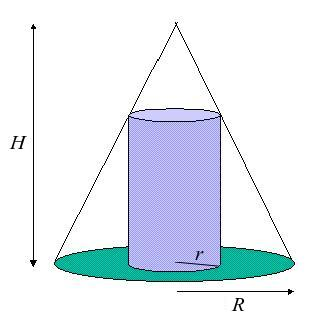
\includegraphics[width=0.4\textwidth]{cylinder}
              \caption{A cylinder inscribed in a cone.\label{fig:cylinder}}
            \end{figure}
    \end{parts}
  \question
    \begin{parts}
      \part Compute the derivatives of the following functions.
        \begin{subparts}
          \subpart[2] $$ y = \frac{e^{-x} + \sin x}{x} $$
          \subpart[1] $$ y = \sqrt{x}\left(x^2 + 5x + \frac{1}{x} \right) $$
        \end{subparts}
      \part
        \begin{subparts}
          \subpart[1] Write down the expression for the derivative of $ x^3 $ from first principles. \textit{You need not evaluate the limit.}
          \subpart[2] Hence, or otherwise, compute the following limit:
            \begin{displaymath}
              \lim_{h \to 0} \frac{(2 + h)^3 - 8}{h}
            \end{displaymath}
        \end{subparts}
      \part[4] Find the interval(s) on which the function $ f $ defined below is concave up.
            \begin{displaymath}
              f(x) = \frac{x^5}{20} - \frac{2x^3}{3} + 16x + 9
            \end{displaymath}
    \end{parts}
  \clearpage
  \question
    \begin{parts}
      \part[2] Show that the rate of change of $ g $ with respect to $ t $ at $ t = 2 $ is $ \frac{3\pi}{2} $ if
            \begin{displaymath}
              g(t) = \sin(\pi\sqrt{3t^2 + 4}).
            \end{displaymath}
      \part[3] Find the equation to the normal line of the curve $ y = x^4 - 3x^3 - 2x^2 + 2x - 1 $ at the point $ (0, -1) $.
      \part[2] Sand is being poured into a hole at a rate of $ \od{S}{t} = 3t + 4 $, and the depth of the hole is
            given by $ h = 12 - \sqrt{S} $. Find $ \od{h}{t} $ in terms of $ t $ and $ S $, and show that $ h $ has
            no maxima or minima at any time after $ t = 0 $.
      \part[3] Show that $ y = 2x^3 - 18x^2 + 90x + 3 $ has no tangent line with a slope of 3.
    \end{parts}
\end{questions}
\end{document}
